\subsection{Questão 18}

\subsubsection{Enunciado}

A Fig.~\ref{fig:34-36} mostra a ampliação lateral \(m\) de um objeto em função da distância \(p\) do objeto em relação a um espelho esférico quando o objeto é deslocado ao longo do eixo central do espelho.

A escala do eixo horizontal é definida por
\[
p_s = 10{,}0\,\text{cm}.
\]

Qual é a ampliação do objeto quando este se encontra a \(21\,\text{cm}\) do espelho?

\begin{figure}[h]
    \centering
    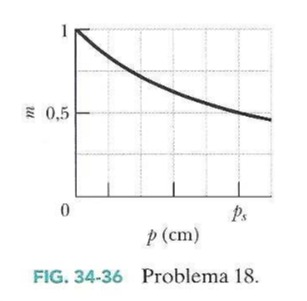
\includegraphics[width=0.40\textwidth]{figures/fig34-36.jpeg}
    \label{fig:34-36}
\end{figure}

\subsubsection{Resolução}
\textbf{Resolução}

Pelo gráfico, observa-se que:

\[
m = 1 \quad \text{quando} \quad p = 0,
\]

e

\[
m \approx 0{,}45 \quad \text{quando} \quad p = p_s = 10\,\text{cm}.
\]

Para um espelho esférico convexo, a ampliação lateral é dada por

\[
m=\frac{f}{p+f}.
\]

Utilizando o ponto \(p=10\,\text{cm}\) e \(m\approx 0{,}45\), temos:

\[
0{,}45=\frac{f}{10+f}.
\]

Multiplicando ambos os lados por \((10+f)\):

\[
0{,}45(10+f)=f.
\]

Desenvolvendo:

\[
4{,}5+0{,}45f=f.
\]

Logo,

\[
4{,}5=0{,}55f,
\]

e

\[
f\approx 8{,}18\,\text{cm}.
\]

Para \(p=21\,\text{cm}\), a ampliação será

\[
m=\frac{8{,}18}{21+8{,}18}.
\]

Assim,

\[
m\approx \frac{8{,}18}{29{,}18}
\approx 0{,}28.
\]

Portanto, a ampliação do objeto quando ele se encontra a \(21\,\text{cm}\) do espelho é

\[
\boxed{m \approx 0{,}28}.
\]

\vspace{1cm}
